\newpage
%

\chapter{Compiling and running OASIS3}
\label{sec_compilationrunning}

\section{Compiling OASIS3 and TOYCLIM}
\label{subsec_compile}

Compiling OASIS3 and TOYCLIM (see section \ref{subsec_toyclim})
can be done using the top makefile \newline {\tt TopMakefileOasis3} and
platform dependent header files as described in section
\ref{sec_notSCE}. Note OASIS3 is temporarily
released without the corresponding PRISM Standard Compile Environment
and Running Environment (SCE/SRE); they will be included when the
migration from CVS to Subversion will be realized in CERFACS.

%For both methods, the same low-level makefiles in each source
%directory are used. 
During compilation, a new directory branch is
created {\tt /prism/{\it arch}}, where {\it arch} is the name of the
compiling platform architecture (e.g. {\it Linux}).  After successful
compilation, resulting executables are found in {\tt /prism/{\it
    arch}/bin}, libraries in {\tt /prism/{\it arch}/lib} and object
and module files in {\tt /prism/{\it arch}/build}.

The different pre-compiling flags used for OASIS3 and its associated
PSMILe library are described in section \ref{subsec_CPP}.

\subsection{Compilation with TopMakefileOasis3}
\label{sec_notSCE}

Compiling OASIS3 and TOYCLIM using the top makefile {\tt
  TopMakefileOasis3} can be done in directory {\tt
  prism/src/mod/oasis3/util/make\_dir}. {\tt TopMakefileOasis3} must
be completed with a header file {\tt make.{\it your\_platform}}
specific to the compiling platform used and specified in \\{\tt
  prism/src/mod/oasis3/util/make\_dir/make.inc}.  One of the files
{\tt make.pgi\_cerfacs}, {\tt make.sx\_frontend} or {\tt make.aix} can
by used as a template.  The root of the prism tree can be anywere and
must be set in the variable {\tt PRISMHOME} in the {\tt make.{\it
    your\_platform}} file. The choice of MPI1, MPI2 or NONE
(interpolator-only mode, see section \ref{subsec_interpolator}) is
also done in the {\tt make.{\it your\_platform}} file (see {\tt
  \$CHAN} therein).

The following commands are available:

\begin{itemize}
\item {\tt make -f TopMakefileOasis3} 

  compiles OASIS3 libraries {\it clim}, {\it anaisg}, {\it anaism},
  {\it fscint}, {\it scrip} and creates OASIS3 main executable {\tt
    oasis3.\$CHAN.x} (where {\tt \$CHAN} is {\tt MPI1}, {\tt MPI2} or
  {\tt NONE}) ;

\item {\tt make -f TopMakefileOasis3 toyclim}

  compiles OASIS3 libraries as above, compiles {\it mpp\_io} and {\it
    psmile} librairies, and creates OASIS3 and TOYCLIM executables
  oasis3.MPI[1/2].x, toyatm.MPI[1/2].x, toyoce.MPI[1/2].x and
  toylan.MPI[1/2].x ;

\item {\tt make clean -f TopMakefileOasis3}: 

  cleans OASIS3 and TOYCLIM compiled files, but not the libraries ;

\item {\tt make realclean -f  TopMakefileOasis3}: 

  cleans OASIS3 and TOYCLIM compiled files including libraries.

\end{itemize}

Log and error messages from compilation are saved in the files
COMP.log and COMP.err in make\_dir.

\subsection{CPP keys}
\label{subsec_CPP}

The following CPP keys are coded in OASIS3 and associated PSMILe library and
can be specified in {\tt CPPDEF} in {\tt make.{\it your\_platform}} file.

\begin{itemize}

\item To indicate which communication technique will be used
  (see sections \ref{subsubsec_Initialisation} and \ref{subsec_namcouplefirst}):

  \begin{itemize}
  \item {\tt use\_comm\_MPI2} (by default): CLIM/MPI2 
  \item {\tt use\_comm\_MPI1} : CLIM/MPI1
  \item {\tt use\_comm\_NONE} : no communication technique for Oasis
    (interpolator-only mode NONE)
  \end{itemize}
  The SIPC, PIPE and GMEM communication techniques available in
  previous versions should still work but are not maintained anymore
  and were not tested.

\item To indicate the precision for REAL variables:

  \begin{itemize}
  \item {\tt use\_realtype\_double} (by default): to exchange double
    precision coupling fields declared as {\tt
      REAL(kind=SELECTED\_REAL\_KIND(12,307))}
  \item {\tt use\_realtype\_single}: to exchange single precision coupling
    fields declared as \newline {\tt REAL(kind=SELECTED\_REAL\_KIND(6,37))}
  \end{itemize}
  Note that if {\tt use\_realtype\_single} is activated the compiling
  option promoting reals should be removed from {\tt F90FLAGS}.

\item When linking OASIS3 and PSMILe with a netCDF library which is
  highly recommended\footnote{Linking with netCDF is mandatory when
    using SCRIPR transformations (see section \ref{subsec_interp}).}
  (the opposite case should work but was not fully tested): 
  \begin{itemize}
  \item{\tt use\_netCDF}
  \end{itemize}

\item Mandatory for compiling the {\it mpp\_io} and {\it psmile}
  libraries:
  \begin{itemize}
  \item{\tt use\_libMPI}
  \end{itemize}

\item Mandatory for compiling the {\it mpp\_io} library if LAM
  implementation of MPI is used:
  \begin{itemize}
  \item{\tt use\_LAM\_MPI}
  \end{itemize}

\item For more information in log files {\it *.prt*} during the psmile
  library exchanges:
  \begin{itemize}
  \item{\tt \_\_VERBOSE}
  \end{itemize}

\item For more debugging information to the standard output from the
  {\it mpp\_io} library:
  \begin{itemize}
  \item{\tt DEBUG}
  \end{itemize}

\item The CPP key {\tt \_\_DEBUG} can also be activated for:

  \begin{itemize}
  \item deadlock detection in {\it clim} and {\it psmile} librairies;
  \item more debugging information in log files {\it *.prt*} during
    the {\it psmile} library I/Os;
  \item in SCRIPR vector transformation, for writing the resulting
    vertical component in the spherical coordinate system after
    interpolation to a file {\tt projection.nc} (see section
    \ref{subsec_interp}).
  \end{itemize}

\item To compile the PSMILe communication library without the I/O
  functionality (see section \ref{subsec_namcouplesecond}), i.e to
  compile only empty routines in {\tt prism/src/lib/mpp\_io}:
  \begin{itemize}
  \item{\tt key\_noIO}
  \end{itemize}

\item For compiling without linking the SCRIP library:
  \begin{itemize}
  \item {\tt key\_noSCRIP}
  \end{itemize}

\item Other platform dependent CPP keys, that should be automatically
  activated on the corresponding platforms, are defined and used in {\tt
    prism/src/lib/mpp\_io/include}

\end{itemize}

%\subsection{Compilation using the PRISM Standard Compiling Environment (SCE)}
%\label{sec_SCE}
%
%
%
%
%XXXX a revoir XXX
%
%OASIS3 and the TOYCLIM coupled model use the PRISM standard directory
%structure (see also \cite{leg04}) and Standard Compiling Environment (see
%also \cite{gay04}). To
%compile OASIS3 and toyatm, toyoce and toyche component models, one
%should go through the following steps:
%\begin{enumerate}
%\item Go in the directory {\tt prism/util/compile/frames}.
%
%\item Create the include files for your platform if they do not
%already exist in directory \break {\tt
%prism/util/compile/frames/include\_<node>} where {\tt <node>} is the
%name of the platform. 
%
%\item Generate a compile script for the libraries using the script
%Create\_COMP\_libs.frm:
%
%\vspace*{2ex}
%\begin{Frame}
%  \vspace*{1ex}
%  \Unixcmd{Create\_COMP\_libs.frm "" "" "" ""}
%\end{Frame}
%\vspace*{2ex}
%
%The first parameter can be either {\tt ""} or {\tt "-"} to direct the
%standard output to a file or the screen.
%
%The second parameter an be either {\tt ""}, {\tt "-"} or {\tt "+"} to
%direct the standard error to a file, the screen or the standard
%output.
%
%If the compile scripts shall be created for another platform than the
%one where the \break Create\_COMP\_libs.frm script is launched, the third
%parameter has to contain the abbreviated node name ``node".
%
%The compile script for the libraries \texttt{COMP\_libs.$<$node$>$}
%should then be created in the directory \texttt{prism/util}.
% 
%\item Generate a compile scrip for OASIS3 and for each of the component
%models using the script Create\_COMP\_models.frm:
%\vspace*{2ex}
%\begin{Frame}
%  \vspace*{1ex}
%  \Unixcmd{Create\_COMP\_models.frm oasis3 "mp" "" "" "" }\\
%  \Unixcmd{Create\_COMP\_models.frm toyoce "mp" "" "" "" "ID" "toyatm toyoce toyche"}\\
%  \Unixcmd{Create\_COMP\_models.frm toyatm "mp" "" "" "" "ID" "toyatm toyoce toyche"}\\
%  \Unixcmd{Create\_COMP\_models.frm toyche "mp" "" "" "" "ID" "toyatm toyoce toyche"}
%\end{Frame}
%\vspace*{2ex}
%
%The second parameter ``mp'' specifies the message passing used, which
%determines how the models are launched (see also section
%\ref{subsubsec_Initialisation}).  If the default `MPI2' is chosen, the
%string has to be empty (specification of MPI2 results in an error);
%otherwise, MPI1 has to be given, or NONE for the interpolator only
%mode -see section \ref{subsec_interpolator}.  The OASIS3 executable
%will have the string MPI1 or MPI2 appended to its name. The 3 toy
%models can also be compiled with either the MPI1 option or the default
%MPI2 option (empty string).
%
%The third parameter can be either {\tt ""} or {\tt "-"} to direct the
%standard output to a file or the screen.
%
%The fourth parameter an be either {\tt ""}, {\tt "-"} or {\tt "+"} to
%direct the standard error to a file, the screen or the standard
%output.
%
%If the compile scripts shall be created for another platform than the
%one where the \break Create\_COMP\_models.frm script is launched, the fifth
%parameter has to contain the abbreviated node name ``node".
%
%The sixth parameter ``ID'' is version acronym for differentiation of
%executables (not relevant for OASIS3 and TOYCLIM toy models).
%
%Finally the last parameter gives the name of all the component models
%in the coupled constellation. This list is not relevant for OASIS3,
%but it has to be given for the toymodels. The specified partner models
%are checked against allowed partners and no default is set.
%
%The scripts to compile OASIS3 and the 3 toy coupled models,
%\texttt{COMP\_oasis3\_<mp>.<node>}
%\texttt{COMP\_toyatm\_<ID>.<node>}, \texttt{COMP\_toyoce\_<ID>.<node>},
%\texttt{COMP\_toyche\_<ID>.<node>} should then be created, respectively in
%directories \texttt{prism/src/mod/oasis3}, \texttt{ /toyatm},
%\break \texttt{ /toyoce}, \texttt{ /toyche}. 
%
%\item The compilation scripts created can now be used to compile
%OASIS3 and the 3 toy models. All four compile scripts have then to be
%launched explicitely by the user in their respective directory. 
%\vspace*{2ex}
%\begin{Frame}
%  \vspace*{1ex}
%  \Unixcmd{COMP\_oasis3\_<mp>.<node>}\\
%  \Unixcmd{COMP\_toyatm\_<ID>.<node>}\\
%  \Unixcmd{COMP\_toyoce\_<ID>.<node>}\\
%  \Unixcmd{COMP\_toyche\_<ID>.<node>}
%\end{Frame}
%\vspace*{2ex}
%
%The scripts compile the models with the MPI library specified during
%their generation.  The script that triggers the update of the
%libraries, \texttt{COMP\_libs.$<$node$>$}, is automatically called by
%the model compilation scripts for the librairies they need. Libraries
%needed by OASIS3 are anaisg, anaism, scrip, fscint, and clim for MPI1
%and MPI2 mode (clim is not compiled in NONE mode). The toy
%models need psmile and mpp\_io.
% 
%\item The result should be executables {\tt oasis3.<mp>.x}, {\tt
%toyatm.<mp>.x}, {\tt toyoce.<mp>.x}, and {\tt toyche.<mp>.x} in the
%{\tt \$BLDROOT/bin} directory defined by the compile scripts, where
%{\tt <mp>} is either MPI1 or MPI2.
%
%\end{enumerate}

\section{Running OASIS3 in coupled mode with TOYCLIM}
\label{sec_coupled_mode}

In order to test the OASIS3 coupler in a light coupled configuration,
CERFACS has written 3 ``toy'' component models, mimicking an
atmosphere model (toyatm), an ocean model (toyoce), and a
chemistry model (toyche). These ``toy'' component models
are `empty' in the sense that they do not model any real physics or
dynamics. The coupled combination of these 3 ``toy'' component models
through OASIS3 coupling software is refered to as the TOYCLIM coupled
model; the TOYCLIM coupling is realistic as the coupling algorithm
linking the toy component models, the size and the grid of the
2D coupling fields, and the operations performed by
OASIS3 on the coupling fields are realistic.

The current version of OASIS3 and its TOYCLIM example coupled model
was successfully compiled and run on NEC SX6, IBM Power4, and Linux PC
DELL, and previous versions were compiled and run on many other platforms.

Compiling OASIS3 and TOYCLIM was described in section
\ref{subsec_compile}. In the following section, the TOYCLIM example
coupled model is first described in more detail (see section
\ref{subsec_toyclim}), then instructions on how to run TOYCLIM are
given in section \ref{subsec_running_toyclim}.

\subsection{TOYCLIM description}
\label{subsec_toyclim}

\subsubsection{The toyoce model}
\label{sec:toyoce}

The toyoce model, which sources can be found in
{\tt prism/src/mod/toyoce/src}, has a 2D logically-rectangular, streched
and rotated grid of 182x152 points, which corresponds to a real ocean
model grid (the pole of convergence is shifted over Asia). Toyoce timestep is
14400 seconds; it performs therefore 36 timesteps per 6-day run.

OASIS3 PRISM System Model Interface (PSMILe) routines are detailed in
section \ref{sec_modelinterfacing}. At the beginning of a run, toyoce
performs appropriate PSMILe calls to initialize the coupling, define
its grids, and declare its I/O or coupling fields. As toyoce is not
parallel, it calls the PSMILe prism\_def\_partition routine to
define only one Serial partition containing the 182X152 grid points.

Then, toyoce starts its timestep loop. At the beginning of its timestep,
toyoce calls the PSMILe prism\_get routine 7 times to request the
fields named Field3 to Field9 on table \ref{tab:couplingIOfields}. At
the end of its timestep, toyoce calls PSMILe prism\_put routine to send
fields named Field1 and Field2 on table
\ref{tab:couplingIOfields}. The fields will be effectively received or
sent only at the coupling frequency defined by the user (see section
\ref{subsec_namcouplesecond}). As toyoce contains no real physics or dynamics,
it defines a simple feed back between Field1 and Field3 and between
Field2 and Field7 such as:
$$ Field1 = Field3 + 1 $$
$$ Field2 = Field7 + 1 $$

Finally, at the end of the run, toyoce performs the PSMILe finalization call. 

\subsubsection{The toyatm model}
\label{sec:toyatm} 

The toyatm model, which sources can be found in
{\tt prism/src/mod/toyatm/src}, has a realistic atmospheric T31 Gaussian
grid (96x48 points). Its timestep is 3600 seconds; it therefore performs 144
timesteps per 6-day run.

As toyoce, toyatm performs, at the beginning of a run, appropriate
PSMILe calls to initialize the coupling, define its grids, and declare
its I/O or coupling variables. Then toyatm retrieves a local
communicator for its internal parallelization with a call to PSMILe
prism\_get\_localcomm routine, useful if the {\tt MPI1} communication
technique is chosen by the user (see section
\ref{subsubsec_Initialisation}). Toyatm can run on 1 or 3 processes,
depending on the variable {\tt il\_nbcplproc} (hardcoded to 3 by
default). If the user modifies this variable and hardcodes {\tt
  il\_nbcplproc = 1}, toyatm runs on only one process and defines only
one Serial partition containing the 96X48 grid points. If {\tt
  il\_nbcplproc = 3}, toyatm runs on 3 processes and its decomposition
depends on the {\tt cdec} parameter, hardcoded to {\tt APPLE}. In this
case, each of the 3 toyatm processes calls the PSMILe
prism\_def\_partition routine to define 1 segment of an APPLE
decomposition (1536 grid points per segment). If the user changes the
hardcoded value of {\tt cdec} to {\tt BOX}, each process will define 1
`box' of a BOX decomposition; the first two processes treat a box of
64X24 points, while the third process treats a box of 128X12 points.
If the user hardcodes {\tt cdec=`ORANGE`}, each process will define a
partition of two segments of 768 points distant of 1536 points.

Then, toyatm starts its timestep loop. At the beginning of its timestep,
toyatm calls the PSMILe prism\_get routine 3 times to request the fields
named Field1, Field2 and Field11 on table
\ref{tab:couplingIOfields}. At the end of its timestep, toyatm calls
PSMILe prism\_put routine to send  fields named Field4 to Field10 on
table \ref{tab:couplingIOfields}. The fields will be effectively
received or sent only at the coupling frequency defined by the user
(see section \ref{subsec_namcouplesecond}). As toyatm contains no real physics
or dynamics, it defines a simple feed back between the different
fields as:

$$ Field5 = Field1 + 1  $$
$$ Field7 = Field2 + 1 $$
$$ Field10 = Field11 + 1 $$
$$ Field4 = Field1 + 1 $$
$$ Field8 = Field2 + 1 $$
$$ Field6 = Field1 + 1 $$
$$ Field9 = Field2 + 1 $$

Finally, at the end of the run, toyatm performs the PSMILe finalization call.

\subsubsection{The toyche model}
\label{sec:toyche} 

Toyche, which sources can be found in {\tt prism/src/mod/toyche/src},
is integrated on the same atmospheric model grid than toyatm. Its
timestep is 7200 seconds; it therefore performs 72 timesteps per 6-day
run.

As the other toymodels, toyche performs, at the beginning of a run,
appropriate PSMILe calls to initialize the coupling, define its grids,
and declare its I/O or coupling variables; it also retrieves a local
communicator if needed. As toyche has the same grid than toyatm, a direct
exchange of coupling fields can occur between those two models,
without going through OASIS3 interpolation process. To insure this,
the coupling field must have a field status `IGNORED' or `IGNOUT' in
the OASIS3 configuration file {\it namcouple} (see section
\ref{subsec_namcouplesecond}) and the two models must have also the same
parallel decomposition.  Toyche decomposition is hardcoded the same way
than toyatm, and if the user modifies the toyatm decomposition, he has to
modify the toyche decomposition the same way by changing toyche values for {\tt
il\_nbcplproc} and {\tt cdec} (see above for toyatm).

At the beginning of its timestep, toyche calls the PSMILe prism\_get
routine to request Field10 (see table \ref{tab:couplingIOfields}). At
the end of its timestep, toyche calls PSMILe prism\_put routine to send
Field11. As toyche contains no real physics or dynamics, it defines a
simple feed back between Field11 and Field10 such as:
$$ Field11 = Field10 + 1 $$

Finally, at the end of the run, toyche performs the PSMILe finalisation call.

\subsubsection{TOYCLIM coupling algorithm}

 The coupling algorithm between the TOYCLIM component models toyoce, toyatm,
 and toyche is described here.
 
Table \ref{tab:couplingIOfields} lists the coupling fields exchanged
between those 3 model components, giving the symbolic name used in
each component and indicating whether the model produces the field
(src) or receives it (tgt).
 
\vspace*{1ex}
\begin{table}[ht]
	\begin{tabularx}{16cm}[t]{|l|l|l|l|l|X|}
	\hline
	  & 
	 toyoce & 
	 toyatm & 
	 toyche &
	 restart &
	 function \\
	\hline\hline
	 Field1 & 
	 SOSSTSST (src) & 
	 SISUTESU (tgt) &
	 & 
	 fldo1.nc &
	 $F_1$ \\
	\hline
	 Field2 & 
	 SOICECOV (src) & 
	 SIICECOV (tgt) &
	 & 
	 fldo1.nc &
	 $F_1$ \\
	\hline
	 Field3 & 
	 SOALBEDO (tgt) & 
	 & 
	 &
	 SOALBEDO.nc &
	  \\
	\hline
         Field4 & 
	 SONSHLDO (tgt) &
	 CONSFTOT (src) &
	 &
	 flda1.nc &
	 $F_2$ \\
	\hline
         Field5  &    
         {\it SOSHFLDO}&
	 COSHFTOT (src)&
	 &
	 &
	 $F_2$ \\
	\hline
         Field6 &    
         SOWAFLDO (tgt) &
         COWATFLU (src) &
         &
         flda1.nc &
	 $F_2$ \\
	\hline    
         Field7 & 
         SORUNOFF (tgt) &
         CORUNOFF (src) &
         &
         flda1.nc &
	 $F_2$ \\
	\hline    
         Field8 &
         SOZOTAUX (tgt)&
         COZOTAUX (src)&
         &
         flda2.nc &
	 $F_3$ \\
	\hline    
         Field9 &
         SOMETAUY (tgt)&
         COMETAUY (src)&
         &
         flda2.nc &
	 $F_3$ \\
	\hline
	 Field10 &
         &
         COSENHFL (src) &
         SOSENHFL (tgt) &
         flda3.nc &
	 $F_1$ \\
	 \hline
	 Field11 &
         &
         COTHSHSU (tgt)&
         SOTHSHSU (src) &
         flda4.nc &
	 $F_1$ \\
	 \hline	         
	\end{tabularx}
\caption[Coupling and I/O fields of the TOYCLIM coupled model]
	{Coupling and I/O fields of the TOYCLIM coupled model. The
	symbolic name used in each toy model is given and it is
	indicated whether the model produces the field (src) or
	receives it (tgt). The function used to create the field in
	the initial restart file is also given.}
\label{tab:couplingIOfields}
\end{table}
\vspace*{1ex}

Figure \ref{fig:toyclimcouplingalgo} illustrates the coupling
algorithm between the 3 TOYCLIM toy models for $Field_1$, $Field_3$,
$Field_4$, $Field_{10}$, and $Field_{11}$.

$Field_1$ is sent from toyoce component to toyatm component at the
coupling frequency $dtF_1$ defined by the user in the configuring file
{\it namcouple}. As interpolation is
needed between toyoce and toyatm grids, this exchange must go through
OASIS3 interpolation process. In the {\it namcouple}, $Field_1$ field status
must therefore be $EXPORTED$ and the interpolation must be defined. If
the user wants the field to be also automatically written to files
before being sent (below the prism\_put), and after being received (below
the prism\_get), he can choose the field status $EXPOUT$. In toyoce and toyatm
codes, the prism\_put and prism\_get routines are respectively called
every timestep with an argument corresponding to the time at the
beginning of the timestep. The lag of $Field_1$, defined as 4 hours
(14400 seconds) in the {\it namcouple}, is automatically added to the
prism\_put time argument; the prism\_put called at the toyoce timestep
preceeding the coupling period therefore matches the prism\_get called
in toyatm at the coupling period.

At the beginning of the run (i.e. at time = 0), the toyoce prism\_put for
$Field_1$ is not activated (as a positive lag is defined for
$Field_1$) and OASIS3 automatically read $Field_1$ in its coupling
restart file, fldo1.nc, and sends it to toyatm component after
interpolation. The different functions used to create the fields in
the initial restart file are also indicated in table
\ref{tab:couplingIOfields}. They are defined as follows:

$$ F_1 = 2+ cos[\pi * acos(cos(\theta)cos(\phi))] $$
$$ F_2 = 2 + cos^{2}(\theta) cos(2\phi)$$
$$ F_3 = 2 + sin^{16}(2 \phi) cos(16 \phi)$$

$F_1$ represents a global dipole reaching its maximum and minimum
values at the equator, respectively at the date-line and at the
Greenwich meridian. $F_2$ represents two dipoles reaching
respectively their maximum and minimum
values at the equator, respectively at the date-line and at $90^{o}$ W, and at the
Greenwich meridian and at $90^{o}$ E; it is similar to
a spherical harmonic with {\it l} = 2 and {\it m} = 2, where {\it l}
is the sherical harmonic order and {\it m} is the azimuthal wave
number. $F_3$ represents a series of dipoles centered at $45^{o}$ N
and $45^{o}$ S; it is similar to
a spherical harmonic with {\it l} = 32 and {\it m} = 16 and is useful
for testing interpolation of fields with relatively high spatial
frequency and rapidly changing gradients.

The exchange of $Field_2$ from toyoce to toyatm and $Field_4$, $Field_6$,
$Field_7$, $Field_8$ and $Field_9$ from toyatm to toyoce follow exactly the
same logic as for $Field_1$.

$Field_3$ as a status \texttt{INPUT} in the {\it namcouple}. $Field_3$
will therefore not be exchanged between two models but will be read
from a file automatically below the target model toyoce prism\_get
calls, at the user-defined frequency in the input file also specified
in the {\it namcouple}, \texttt{SOALBEDO.nc}.

$Field_5$ as a status of \texttt{OUTPUT} in the {\it namcouple}. It
will therefore be only automatically written to a file at the
user-defined frequency, below the source model toyatm prism\_put calls.  The
name of the file will be automatically composed of the field symbolic
name (here \texttt{COSHFTOT}) and of the begin and end dates of the
run. The prism\_get calls in the toyoce model will not be activated at
all.

$Field_{10}$ and $Field_{11}$ are exchanged respectively from toyatm to
toyche and from toyche to toyatm following $Field_1$ logic described here
above, except that the exchanges take place directly between the
component models without going to OASIS3 interpolation process, as toyatm
and toyche have the same grid and the same parallel partition. The
fields status chosen by the user for those fields in the {\it
namcouple} should therefore be \texttt{IGNORED} (or \texttt{IGNOUT} if
the user wants the fields also automatically be written to files below
the prism\_put and after the prism\_get). At the beginning of the run
(i.e. at time = 0), the toyoce prism\_get called to receive those
fields will automatically read the fields in their corresponding
coupling restart files flda3.nc and flda4.nc.

\vspace*{1ex}
\begin{figure}[htbp]
\epsfig{figure=figures/coupling_algo4.eps,height=0.95\textwidth, angle=270,clip=}
%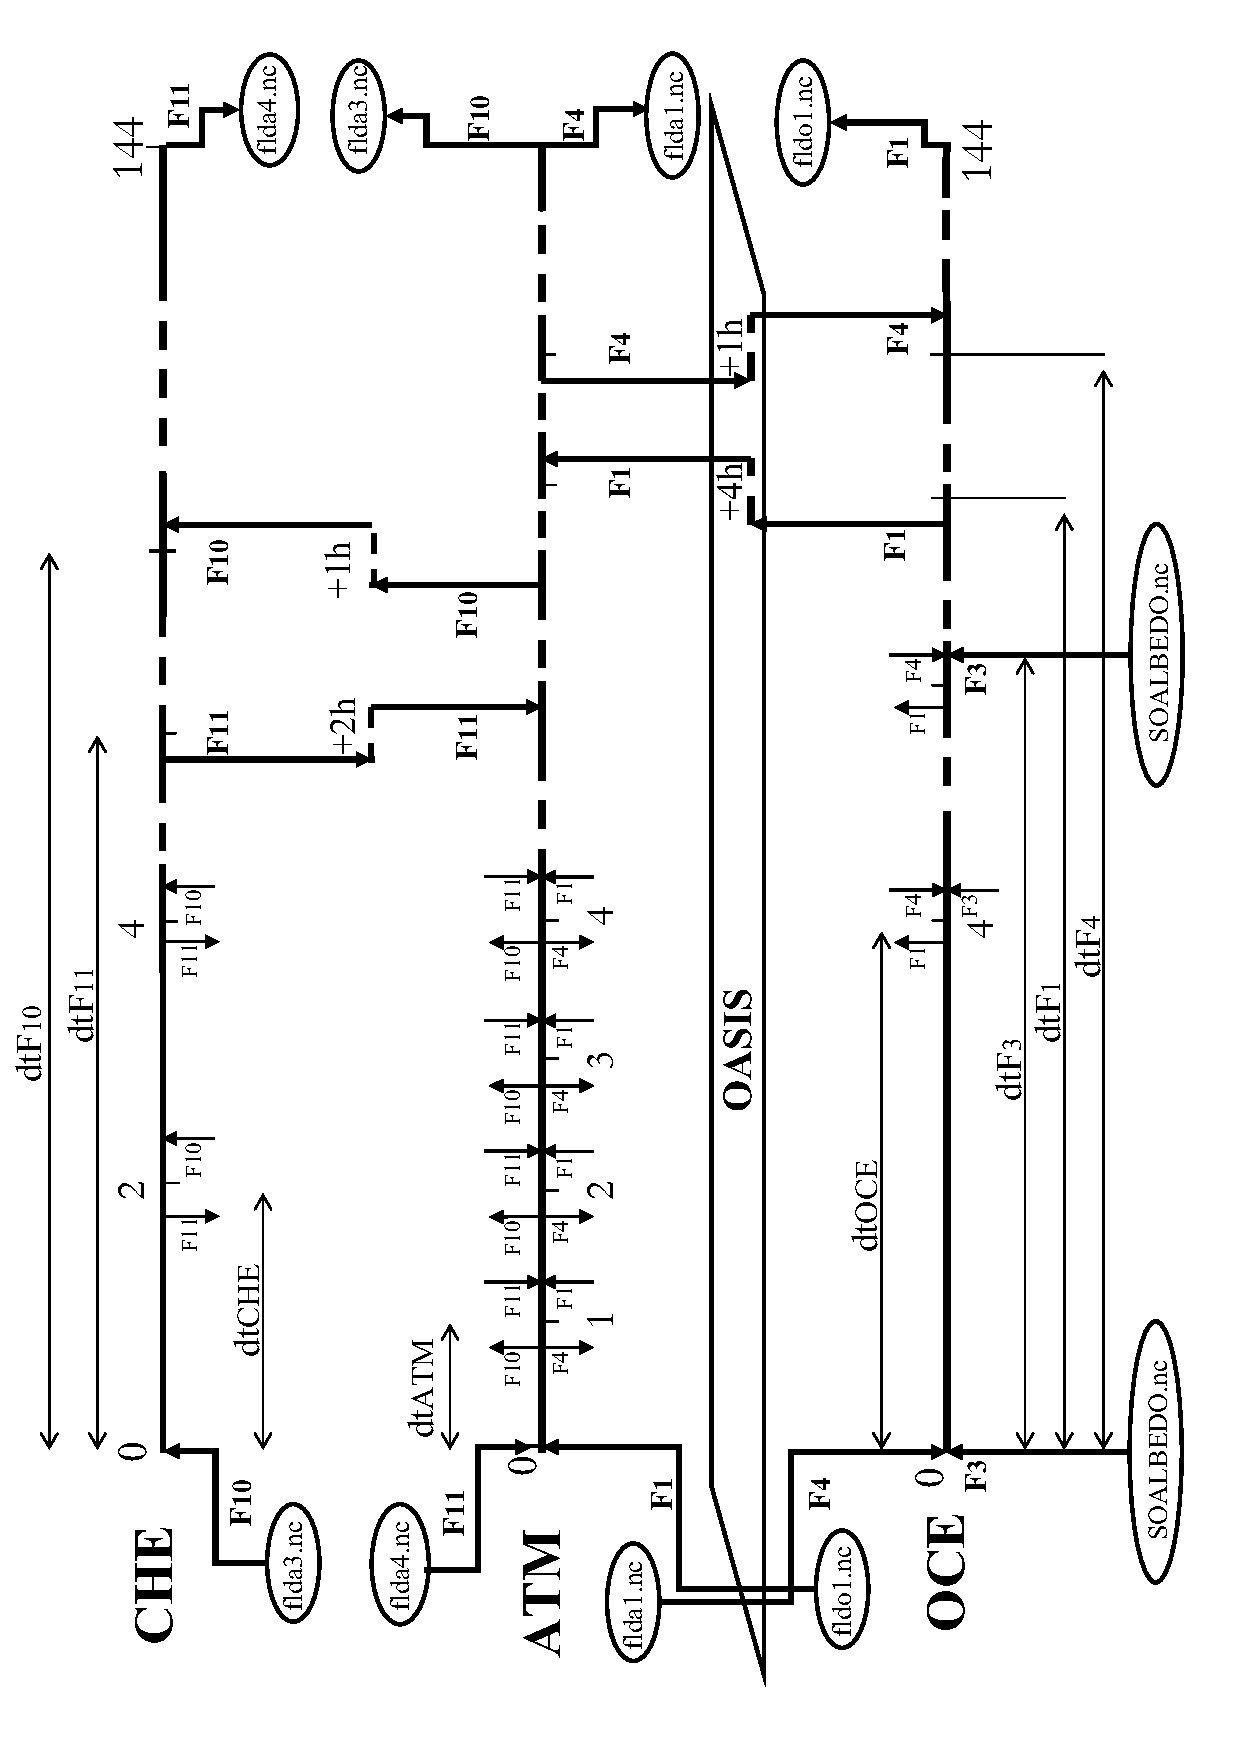
\includegraphics[angle=0,bb=50 0 600 800]{figures/coupling_algo4}
\caption{Exchange algorithm between the 3 TOYCLIM component models for
  fields $Field_1$, $Field_3$,
$Field_4$, $Field_{10}$, and $Field_{11}$. }
\label{fig:toyclimcouplingalgo}
\end{figure}



\subsection{Running TOYCLIM using the script {\tt run\_toyclim}}
\label{subsec_running_toyclim}

Data for running TOYCLIM are contained in tar file {\tt
  input\_toyclim\_standard\_standard\_prism\break \_2-2.tar.gz} or {\tt
  input\_toyclim\_standard\_standard\_prism\_2-2\_single.tar.gz} in
directory {\tt prism/data/toyclim}.  Input files and script are
located in directory {\tt prism/util/running/\break toyclim}.

To run TOYCLLIM, one has to compile OASIS3 and the 3 TOYCLIM component
models (see section \ref{subsec_compile}), to adapt the ``User's
section'' of the running script {\tt
  prism/util/running/toyclim/script/\break run\_toyclim} for his/her
platform, and to launch it.  The script {\tt run\_toyclim} was tested
on Linux PC, NEC SX-6, and IBM Power4.

To run the single precision case, OASIS3 and the 3 component models
have to be compiled in single precision (see section
\ref{subsec_CPP}), the configuration file {\tt
  prism/util/running/toyclim/input/\break namcouple\_single} has to be
renamed {\tt namcouple} (in the same directory, so to be used
automatically), and {\tt comp\_precision=single} has to be specified
in {\tt run\_toyclim}. The configuration file {\tt namcouple\_single}
has to be used because the original {\tt namcouple} specifies some
{\tt MOZAIC} transformations using binary auxiliary files that were
not converted; the results obtained with {\tt namcouple\_single}, into
which the {\tt MOZAIC} transformations are replaced by {\tt
  SCRIPR/DISTWGT} interpolations, will be slightly different.


%\subsection{Running TOYCLIM using the PRISM Standard Running Environment}
%
%XXXX a revoir XXX
%
%{\bf Configuring TOYCLIM using the PRISM SRE}
%%\label{subsec_configuring}
%
%The TOYCLIM example coupled model can be run using the PRISM standard
%running environment (SRE). To do so, one has to go through the
%following steps:
%
%\begin{enumerate}
%\item Go to the directory {\tt prism/util/running/frames}
%\item Create the include files for your platform if they do not
%already exist in directory {\tt
%prism/util\break/running/frames/include\_<node>} where {\tt <node>} is
%the name of the platform.
%\item Run the script Create\_TASKS.frm to generate a setup file for
%your TOYCLIM experiment:
%
%\begin{Frame}
%  \vspace*{1ex}
%  \Unixcmd{Create\_TASKS.frm toyclim <expid>}
%\end{Frame}
%\vspace*{2ex}
%
%where {\tt <expid>} is your experiment name.
%
%\item To change the configuration of your experiment, modify the
%values of the configurable entries in the setup file {\tt
%prism/util/running/frames/setup/setup\_toyclim\_<expid>}, which
%contains default values for these entries. Some of these configurable
%entries directly enter the OASIS3 configuration file {\it namcouple},
%other affect the running script only\footnote{Additional {\it
%namcouple} entries are also configurable by editing directly the
%namcouple base file. Refer to chapter \ref{sec_namcouple} for more
%details.}.  The {\it namcouple} file is created from the {\it
%namcouple} base file (see \texttt{namcouple\_toyclim} in
%\texttt{prism/util/running\break/adjunct\_files/oasis3}) by replacing the
%configurable entries (which begin with "\#") by the value defined in
%the setup file.  The {\it namcouple} will be read by OASIS3 at
%runtime. The variables that can be defined in the set-up file and
%correspond to configurable {\it namcouple} entries are the following:
% 
%\begin{enumerate}
%
%\item{\em jobname}: Experiment identifier; it is composed of three
% digits; ({\em \#Jobname}).
% 
%\item{\em nlogprt}: Integer controlling the amount of information
% written to the OASIS output file {\em cplout}. 0: minimum output, 1:
% medium output, 2: maximum output; ({\em \#Nlogprt}).
%
%\item{\em extrapwr}: Flag to provoke the calculation of weights and
% addresses for nearest neighbour extrapolation (EXTRAP/NINENN) within
% OASIS3 (1) or to read them from file (0); ({\em \#Extrapwr}).
%
%\item{\em stat\_field{\bf xx}}, where {\bf xx} is the number of the
%field in the namcouple: The status of the {\bf xx} coupling/IO field
%can be either `EXPOUT' or `EXPORTED', except for $Field_3$ for which
%it is `INPUT', for $Field_5$ for which it is `OUTPUT' and for
%$Field_{10}$ and $Field_{11}$ for which it is either `IGNOUT' or
%`IGNORED' (see section \ref{subsec_namcouplesecond}); ({\em
%\#Stat\_field{\bf xx}}).
%
%\item{\em dtF{\bf xx}}, where {\bf xx} is the number of the field in
%the namcouple: The coupling or I/O period of the {\bf xx} coupling/IO field,
%which must be a multiple of 14400, except for $Field_3$ for which it
%must be a multiple of 43200, and for $Field_5$, $Field_{10}$ and
%$Field_{11}$ for which it must be a multiple of 3600; ({\em \#Dt{\bf
%xx}}).
%
%\item {\em iniyear}, {\em inimonth} and {\em iniday}: the initial date
%of the experiment, respectively as {\tt YYYY}, {\tt MM} and {\tt
%DD}({\em \#Inidate}).
%
%\item {\em message\_passing}: Message passing method, either MPI2 or
%  MPI1 (for more details, see section \ref{subsubsec_Initialisation});
%  (in {\em \#Channel})
%
%\item {\em bsend}: either `yes' or `no', indicates whether the
% buffered {\tt MPI\_BSend} or the standard blocking send {\tt
% MPI\_Send} will be used to send the coupling fields (for more
% details, see section \ref{subsec_namcouplefirst}) (in {\em \#Channel})
%
%\end{enumerate}
%
%The variables that can be additionally defined in the setup file but
%do not correspond to any
%configurable {\it namcouple} entries are the following:
% 
%\begin{enumerate}
%
%\item {\em ncplvers}: the namcouple version. Put {\tt ""} to use the
%  {\it namcouple} base file completed with the values defined in the
%  setup file. To use another {\it namcouple}, a particular value has
%  to be given to {\em ncplvers}, and a {\it namcouple} named
%  {\tt namcouple\_toyclim\_$<$ncplvers$>$} has to be available in
%  \texttt{prism/util/running/adjunct\_files/oasis3}.
%
%\item{\em gridswr}: either `0' if you want the models to use the grid
%  description files if they exist, or `1' if you want the models to
%  unconditionally (re)generate those grid description files (for more
% details, see section \ref{subsubsec_griddef}).
%
%\end{enumerate}
%
%\item Type {\tt `Create\_TASKS.frm toyclim <expid>'} a second
%time. The script will check the parameters you specified in
%{\tt setup\_toyclim\_<expid>}. If a parameter is not supported or a
%combination of parameters does not make sense Create\_TASKS.frm writes
%an error message and stops.
%\item Correct the experimental setup file if necessary and
%run Create\_TASKS.frm again until the setup check is passed
%successfully.
%
%\end{enumerate}
%
%Once the setup is done, all appropriate files and the script to start
%the experiment are available in the
%directory {\tt $<$home$>$/$<$expid$>$}, where {\tt $<$home$>$} and
%{\tt $<$expid$>$} are
%defined in the setup file.
%
%{\bf Running TOYCLIM using the SRE}
%%\label{subsec_running}
%
%After the setup and configuration phase, the experiment is ready to be
%started with the running script {\tt RUN\_toyclim\_<expid>} in
%directory {\tt $<$work$>$/$<$expid$>$/scripts}, where {\tt $<$work$>$} and
%{\tt $<$expid$>$} are
%as defined in the setup file {\tt setup\_toyclim\_<expid>}.
%
%To run a TOYCLIM experiment, one has to go through the following
%steps:
%
%\begin{enumerate} 
%%\item The file {\tt
%%  toyclim/input\_toyclim\_standard\_\-standard\_prism\_2-1.tar.gz} has
%%  to be copied from the directory {\tt prism/data} to the directory
%%{\tt <archive\_in>/toyclim} on the \break {\tt <archiving\_host>}.  The variables
%%{\tt <archive\_in>} and {\tt <archiving\_host>} are specified in the setup file .
%\item Login on the compute server (if different from the compile server).
%\item Change to the directory {\tt <work>/<expid>/scripts}. 
%\item Submit the runscript {\tt RUN\_toyclim\_<expid>}.
%\end{enumerate}
%
%Running TOYCLIM with the default parameters will result in a 30-day
%experiment executed as five 6-day runs. The final results obtained the
%directory {\tt <work>/<expid>/work} should match the ones in {\tt
%prism/data/toyclim/outdata}. Intermediate results are also saved in
%different sub-directories :
%\begin{itemize} 
% \item the OASIS3 log files of each
%run in {\tt <data>/<expid>/log } or {\tt  <archive>/<expid>/log }
% \item the output netCDF files containing the {\tt EXPOUT} fields in {\tt
%<data>/<expid>/outdata/oasis3 } or {\tt
% <archive>/<expid>/outdata/oasis3 }
%\item the coupling restart files in {\tt  <data>/<expid>/restart } or
%  {\tt  <archive>/<expid>/restart}.
%\end{itemize}
%where {\tt <data>} and {\tt <archive>} are
%defined in the runscript {\tt RUN\_toyclim\_<expid>}.
%
\section{Running OASIS3 in interpolator-only mode}

OASIS3 can be used in an interpolator-only mode, in which case it
transforms fields without running any model (see section
\ref{subsec_interpolator}). Two test-cases are provided with OASIS3 to
illustrate its uses in this mode, the ``testinterp'' test-case (see
section \ref{subsec_running_testinterp}) and the ``testNONE''
test-case (see section \ref{subsec_running_testnone}). 

\subsection{The ``testinterp'' test-case}
\label{subsec_running_testinterp}

The ``testinterp'' test-case can be run to test the interpolation of
different source fields corresponding to analytical functions 
and to evaluate the error between the
interpolated fields and the same analytical functions calculated on the
different target grids.

All files needed to run this test-case can be found in
{\tt prism/data/testinterp/input} and {\tt prism/\break data/testinterp/restart}.

To run ``testinterp'', OASIS3 first has to be compiled in
interpolator-only mode NONE (see section \ref{subsec_compile}). Then
the programs that will calculate the interpolation error, i.e. {\tt
  gen\_error.f90} and {\tt gen\_error\break \_vector.f90} (for vector
fields) in directory {\tt prism/util/running/testinterp/error} have to
be compiled (see script {\tt sc\_comp\_error}).

Then, one has to adapt and execute the running script {\tt
  prism/util/running/testinterp/\break script/sc\_run\_testinterp}.
With {\tt TIME=ONE}, the configuration file {\tt
  prism/data/testinterp/\break input/namcouple\_ONE}, the input files
{\tt flda1.nc, flda2.nc, flda3.nc, fldb1.nc,} \newline {\tt fldo1.nc}
and {\tt fldz1.nc} from {\tt prism/data/testinterp/restart} and the
input files {\tt aaIin.nc} and {\tt caJin.nc} from {\tt
  prism/data/testinterp/restart/vector} are used.  This example also
shows one vector interpolation (field components {\tt a\_at42\_I} and
{\tt c\_at42\_J}).  The test-case automatically writes the error
fields in {\tt error\_*.nc} files and error statistics in {\tt log\_*}
files.

To run the example into which OASIS3 interpolates many time
occurrences from one input file, put {\tt TIME=MANY} in {\tt
  sc\_run\_testinterp}.  The configuration file {\tt
  prism/data/testinterp/input/\break namcouple\_MANY} and the input
file {\tt fldin.nc} in {\tt prism/data/testinterp/restart} is then
used.

The results obtained after running the testinterp test-case should
match the ones in {\tt prism/data/\break testinterp/outdata}.


\subsection{The ``testNONE'' test-case}
\label{subsec_running_testnone}

All files to run the ``testNONE'' test-case can be found in {\tt
  prism/util/running/testNONE}. This test-case provides a flexible
environnement to test the interpolation specified in the {\tt
  INPUT/namcouple} configuration file from a source grid to a target
grid, both grids being defined in regular OASIS3 grid data files {\it
  grids.nc}, {\it masks.nc}, {\it areas.nc} (see section
\ref{subsec_griddata}). 

To run ``testNONE'', the user has to adapt the ``User specifications''
part of the running script {\tt sc\_run\_NONE}. In particular, he has
to specify the directory for the grid data files, the directory for
the {\tt namcouple} and {\tt cf\_name\_table.txt} files, the source
and target grid prefixes in the {\tt namcouple} and in the grid data
files (see section \ref{subsubsec_secondEXPORTED}), an analytic
function, and whether or not the error on the target grid will be
calculated on all points ({\tt MASKERROR=NOT}) or only on non masked
points ({\tt MASKERROR=YES}).

When launched, the running script {\tt sc\_run\_NONE}:
\begin{itemize}
\item creates a working directory
\item compiles and runs the program {\tt
    PROG/create\_inputfield.f90} that creates an input field using the
  chosen analytical function on the specified source grid in file
  {\tt fldin.nc}
\item copy all required input and data file to the working directory 
\item run oasis3 that interpolates the analytical field from {\tt
    fldin.nc} with the interpolation specified in the {\tt namcouple}
\item compile and run the program {\tt PROG/create\_errorfield.f90}
  that calculates the error between the resulting interpolated field
  and the field defined by the chosen analytical function on the
  specified target grid, and writes it to the file {\tt error.nc}
\end{itemize}


